\chapter{Proposed approach}
\label{chapter:proposedApproach}

For solving the problem of detecting malicious PDF documents, we came with a Machine Learning based approach. We took into account the importance of keeping the documents content confidentiality, as well as the need for ensuring the speed of analysis process. This solution will be next integrated into a Cloud framework responsible for remote documents scanning.

\section{Dataset}
\label{section:dataset}
The first step in building the optimal \textit{ML} model was to create a dataset which would train the classifier. Our target was to collect malicious and benign PDF samples used in real life scenarios. Circa 70\% of the clean and malicious documents were downloaded from the online malware repository \textit{Contagio} \cite{contagio}, which provides samples collected from various open sources. Nevertheless, for more recent malicious PDFs we used VirusTotal \cite{virustotal}, Hybrid Analysis \cite{hybridanalysis} and VirSCAN \cite{virscan}, that allow searching files by their hash (\textit{MD5}, \textit{SHA1}, \textit{SHA256}). Some of them provide access to the entire file collection so that we can order them by upload date and search for the most recent uploaded harmful files. Many clean samples were collected from public sources using Google Search Operators, i.e., \code{filetype:pdf}, for restricting search results of PDF files. Additionally, we completed the dataset with more than 100 clean interactive PDF files, that contain embedded 3D Widgets, incorporated JavaScript games etc. These clean samples should train the ML model, so as to correctly classify files even in corner cases. 

\begin{table}[H]
	\caption{Dataset of PDF samples}
	\label{table:pdfSamples}
        \centering
            \begin{tabular}{p{2.5cm} p{9.5cm}}
                \toprule
                
				\textbf{Category} & \textbf{Source} \\
				\hline 
                \texttt{benign} & Contagio, Google Queries, Tetra4D, PdfScripting \\
                \hline
				\texttt{malicious} & Contagio, VirusTotal, Hybrid Analysis, VirSCAN \\
                
                \bottomrule
			\end{tabular}
\end{table}

\section{Proof of Concept}
\label{section:poc}

In the following subsections we will touch upon algorithms and techniques we have used to achieve the purpose of this thesis, namely detecting malicious PDF documents using a Machine Learning based solution. Figure \ref{mlsteps} represents the entire process which was followed while developing the \textit{ML} model. Each process phase will be fathomed in the following.

\begin{figure}[H]
	\centerline{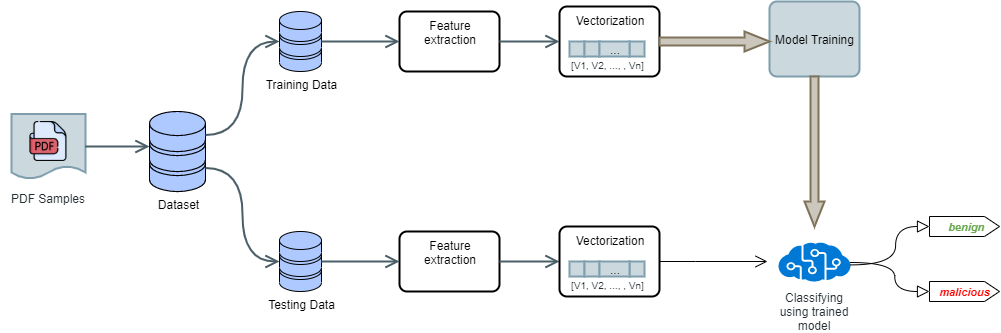
\includegraphics[scale=0.5]{figures/ml.png}}  
	\caption{Machine Learning model creation}
	\label{mlsteps}
\end{figure}

\subsection{Feature Selection}

\subsection{Classification Techniques}
\subsection{Performance Evaluation}
\subsection{Experiment}     % Metasploit + Kali

\section{Used technologies}
\label{section:technologies}
\subsection{Microsoft .NET Framework}
\subsection{PDF Tools and Metasploit Framework}
\cite{zeltser}
\subsection{Python Flask}
\subsection{Scikit-learn Machine Learning Library}
\cite{mlCookbook} 
\subsection{ReactJS Framework}
